\documentclass[sigconf]{acmart}

\usepackage{tabulary}

%% \BibTeX command to typeset BibTeX logo in the docs
\AtBeginDocument{%
  \providecommand\BibTeX{{%
    Bib\TeX}}}

\begin{document}

\title{Realisierung eines Konzepts für eine bedarfsgerechte Datenaufbereitung}

\author{Ahmed Rezk}
\email{st163697@stud.uni-stuttgart.de}

\author{Luke Mayr}
\email{st177937@stud.uni-stuttgart.de}

\author{Metin Arab}
\email{st178931@stud.uni-stuttgart.de}

\author{Tabea Steeb}
\email{st156637@stud.uni-stuttgart.de}

\begin{abstract}
\end{abstract}

\keywords{Data Lake, data preprocessing, ontology, BARENTS, LALO}

\maketitle

\section{Introduction}


\section{BARENTS}
The following section is mainly based on \cite{barents21} and \cite{barents22}.
\subsection{Overview BARENTS}
\subsection{Use case scenario: nut allegens in chocolate samples}


\section{Requirement Specification}
\begin{enumerate}
\item[(R1)] Our goal is an Easy-to-use GUI for domain experts, with which they can create ontologies.
%% TODO: hier statt \cite{barents21} die Stelle im Kapitel Barents angeben
\item[(R2)] Transformations I - III as defined in \cite{barents21} (namely filter, map and reduce operator) are functioning.
\item[(R3)] Created ontologies can be saved.
\item[(R4)] Has a data-processing-engine, which processes data according to the ontology.
\item[(R5)] Our prototype should be functioning with at least one database type. We chose relational databases, since we are most familiar with that.
\end{enumerate}


\section{Related Work}
%% dieses Kapitel optional
Stach et al.~\cite{barents21}


\section{Implementation}

\subsection{Discussion on own implementation vs. existing tools}

\subsubsection{OWLGrEd}
OWLGrEd \cite{owlgred} is a free graphical editor for OWL ontologies in UML style \cite{owlgredW3}. 
It has classes and different connections, including (directed) associations. 
The classes we could modify for the data source and data sink and the association for the data transformations. 
However, this modification would be very time-consuming: classes somehow need to connect to the data source or sink, connections should have different types according to the transformations (filter, map, reduce), and the whole toolbar should be slimmed down to only the necessary tools. 

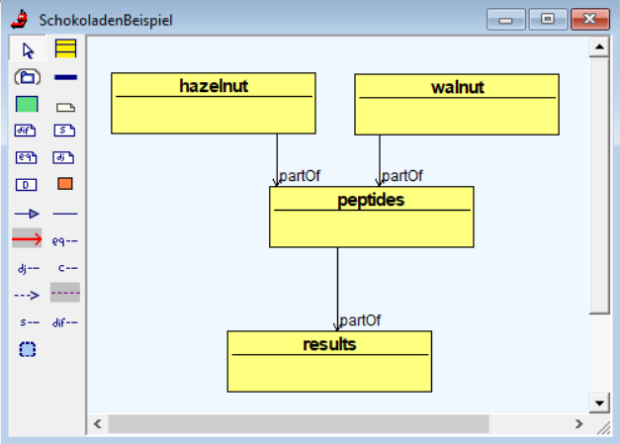
\includegraphics[width = \linewidth]{Owlgred.png}
OWLGrEd already has a function to save the created ontology as a RDF/XML file (*.owl). But here as well would we need to modify a lot such that the RDF/XML file suits the BARENTS model. 

The code is written in Lua (which we are not familiar with) and is difficult to understand (lots of code, with unclear structure, often not or in different languages commented). 

All in all it would be much work to alter the editor to our needs.

\subsubsection{WebVowl}
WebVowl creates and edits ontologies, using a GUI, which simplifies the ontology modeling process.
It has no drag-and-drop funtionality, it, instead,  creates components on-double-click.
Its both possesses import and export functions.
However, it can only export TTL-files.
Jet it is fixable due to the possibility of auto-converting TTL- to XML-/RDF-files using the tool Apache Jena.

Our problem with WebVowl was that there is a lack of information about the structure of the code.
This lack of context made it really difficult, for us, to edit or extend the source code.
\subsubsection{Protégé}
\subsubsection{CoModIDE}
\subsubsection{implementing ourselves}
\subsection{evaluation}

\begin{table} [h]
    \centering
    \begin{tabulary} {\paperwidth} {p{1,5cm}|p{2,5cm}|p{1,3cm}|p{2,5cm}}
        Editor & design & language, Tools & Output \\ \hline
        OwlGrEd & has classes and connections & Lua, lQuery & you can save the created Ontology as RDF/XML file \\ \hline
        WebVowl & & & \\ \hline
        Protégé & & & \\ \hline
        CoModIDE & & & \\ \hline
    \end{tabulary}
\end{table}


\section{Prototyping}
    \subsection{Scope of the Prototype}
        Our prototype is supposed to be a proof of concept for the utility of a GUI that allows users to create a configuration file following the BARENTS specifications. 
        It is worth noting that BARENTS was conceived for the purpose of data provisioning in data lakes.
        Our prototype will only support data provisioning in select relational databases. 
        This allows for both the desired proof of concept, while keeping the scale much for feasible.

    \subsection{Data Access and the Expanded BARENTS Ontology}
        In the BARENTS ontology as described by Stach et al.~\cite{barents21} data features are represented by resources in the ontology.
        This by itself doesn't allow for data access, as metadata such as access credentials and its storage location are missing.  
        The BARENTS zone architecture by Stach et al.~\cite{barents21} contains a Management Zone which provides this information. 
        Later that information is modeled by additional literals in the BARENTS ontology.

        Considering the scope of this project, we opted to omit the Management Zone.
        As such there is no data catalogue for our prototype to reference. 
        Therefore we require the user to provide both a database location, as well as a table within that database. 
        This information is the modeled as two seperate literals.

\subsection{Frontend design}
The user-interface has the minimal size of 900x500 pixels which can be increased into the full screen size of its device.
It is divided into a canvas, making up most of the screenspace, along with a left, right and top bar.
The canvas contains the created graphs.
It is scrollable and plain-white putting the users focus on the graph.
These graphs contain ressources (source, transformation, sink) as nodes and are connected by part-of relationships.
The top bar contains three buttons to import, export (process the created rdf-file) and reset the created graph.
The left sidebar contains the buttons which add the graph-components. 
More specifically, it contains buttons which add ressources and part-of relationships.
The right sidebar contains buttons and texts to name and update selected ressources.

\subsection{Backend}

\section{Evaluation - Requirements Fulfillment}

\section{Conclusion}

%% The next two lines define the bibliography style to be used, and
%% the bibliography file.
\bibliographystyle{ACM-Reference-Format}
\bibliography{references}


\end{document}
\endinput
